% Provenance (never printed): see sources/outline_sources.md (Year 2: palaeogeography through
% the Phanerozoic; sea level; orogenies; mass extinctions and their Earth causes). Maps from the
% plate model of Merdith and others (2021) through the GPlates Web Service; sea level from the
% Miller and others (2005) NOAA study (Haq and others 1987; Kominz and others 2008); flooding and
% the Pitman model after Tasistro-Hart and Macdonald (2023); the big five after Marshall (2023)
% and Kaiho (2022); oceanic anoxic events after Rigo and others (2024) and Walker-Trivett and
% others (2024); CAMP carbon dioxide after Capriolo and others (2020); Chicxulub after
% Pickersgill and others (2026) and Collins and others (2020). Curves and numbers from
% figdata/bachelor-2/phanerozoic.py; exercise and problem values in the Book 4 scratch
% calculator calc/ch19.py.
\chapter{A Terra fanerozoica}\label{ch:b2:phanerozoic-earth}

No oeste do Kansas, no meio da América do Norte, pilares de giz branco erguem-se da
pradaria. O giz é a vasa de um fundo marinho: há cerca de 80 milhões de anos um
mar raso corria de norte a sul através do meio da América do Norte, e as carapaças de
algas flutuantes depositavam-se em seu fundo a alguns centésimos de milímetro por ano. Cinco vezes nos
últimos 540 milhões de anos, uma grande parte das espécies que viviam nesses mares desapareceu num
instante geológico. As duas histórias são da própria Terra: os continentes se moveram e o mar subiu e desceu sobre
eles, e pelo menos três das cinco grandes extinções coincidiram com derrames de lava vindos do interior
do planeta. Este capítulo acompanha o Fanerozoico por seus mapas, seu nível do mar, suas cadeias de
montanhas e suas crises, e põe números em duas delas: com que rapidez as dorsais elevam o mar, e quanta
terra um mar mais alto afoga.
% ledger: kgs:monument-rocks, kgs:chalk, ics:base.Phanerozoic, kaiho22:table, cr03:table

\begin{recall}
\textbf{Dos volumes escolares}: a tectônica de placas e a Pangeia; os fósseis e a escala do tempo
geológico; as transgressões lidas numa falésia. \textbf{Do volume do primeiro ano}: a lei profundidade--idade
do fundo oceânico; a curva hipsométrica; a isostasia; o eustatismo e o nível relativo do mar; as grandes províncias
ígneas; as extinções em massa como marcos estratigráficos, o irídio do limite K--Pg e a
datação da crise do fim do Permiano; os andares e os GSSP. \textbf{Dos capítulos anteriores}: os \omterm{def:b2:alpine-orogen:orogen}{orógenos}
(\cref{ch:b2:alpine-orogen,ch:b2:himalaya-andes}); o \omterm{def:b2:wilson-cycle:wilson}{ciclo de Wilson} e os \omterm{def:b2:wilson-cycle:supercontinent}{supercontinentes}
(\cref{ch:b2:wilson-cycle}); o \omterm{def:b2:basins-compared:backstripping}{backstripping} (\cref{ch:b2:basins-compared}); as bolas de neve do
Criogeniano (\cref{ch:b2:precambrian-earth}). A extinção e a história da vida pertencem aos
livros de biologia; o volume do terceiro ano trata do paleomagnetismo e da estratigrafia de sequências.
\end{recall}

\section{Mapas de um mundo em movimento}\label{sec:b2:phanerozoic-earth:maps}

Uma rocha raramente está onde se formou. Um carvão, um arenito de deserto, um recife: cada um foi depositado a
alguma latitude e tem sido transportado desde então por sua placa. Antes que o clima ou a vida de uma época
passada possam ser lidos nessas rochas, é preciso recolocá-las onde estavam.

\begin{definition}[Paleogeografia; mapa paleogeográfico]\label{def:b2:phanerozoic-earth:palaeogeography}
A \emph{paleogeografia}\index{paleogeografia} é a reconstrução da geografia de uma época
passada: as posições dos continentes e dos oceanos, e de suas linhas de costa, cadeias de montanhas e
mares. Um \emph{mapa paleogeográfico}\index{mapa paleogeográfico} mostra essa geografia numa
época, sobre a grade de latitude e longitude daquela época.
\end{definition}

Quatro tipos de evidência entram num mapa assim. A magnetização das rochas dá a latitude em
que se formaram, o tema do paleomagnetismo no volume do terceiro ano; mas o campo da Terra é
simétrico em torno de seu eixo, de modo que nada diz da longitude. O fundo oceânico registra o movimento das
placas diretamente, por suas faixas magnéticas e suas idades, mas só até o
fundo mais antigo que resta, de cerca de 190 milhões de anos: tudo o que é mais antigo foi subductado. Antes disso,
o encaixe dos continentes, as suturas e os \omterm{def:b2:alpine-orogen:orogen}{orógenos} onde oceanos se fecharam, e os fósseis e
sedimentos que denunciam um clima --- recifes e evaporitos nos trópicos, depósitos glaciais perto dos
polos --- completam o quadro. Os modelos de placas reúnem esses vínculos e fazem cada placa voltar no
tempo; as reconstruções também têm de levar em conta a lenta rotação de toda a Terra sólida em relação
a seu eixo de rotação, chamada deriva polar verdadeira.
% ledger: vh26:palaeogeography, gws:merdith-frame, data:b2-seafloor-age, merdith21:model

\begin{omfigure}
\centering
% figdata/bachelor-2/phanerozoic.py parts map-<t>, cities-<t>, grat (Mollweide, x and y in Earth radii)
\begin{tikzpicture}
\begin{groupplot}[group style={group size=2 by 3, horizontal sep=0.35cm, vertical sep=0.55cm},
  width=0.53\linewidth, axis equal image, hide axis, clip=false,
  xmin=-2.85, xmax=2.85, ymin=-1.43, ymax=1.43,
  title style={font=\small, yshift=-1.5ex}]
\pgfplotsinvokeforeach{500,300,200,100,50,0}{
\nextgroupplot[title={#1~\unit{Ma}}]
\fill[omSea] (axis cs:0,0) ellipse [x radius=2.8284, y radius=1.4142];
\addplot[fill=omLithAlluv!85!black, draw=none] table[x=x, y=y]
  {figdata/out/bachelor-2-phanerozoic-map-#1.dat};
\addplot[black!35, line width=0.2pt] table[x=x, y=y] {figdata/out/bachelor-2-phanerozoic-grat.dat};
\draw[black!70, line width=0.4pt] (axis cs:0,0) ellipse [x radius=2.8284, y radius=1.4142];
\addplot[only marks, mark=*, mark size=1.3pt, red!75!black, point meta=explicit symbolic,
  nodes near coords, nodes near coords style={font=\tiny\bfseries, anchor=south west,
  inner sep=0.5pt, text=red!60!black}]
  table[x=x, y=y, meta=tag] {figdata/out/bachelor-2-phanerozoic-cities-#1.dat};
}
\end{groupplot}
\end{tikzpicture}
\par\smallskip{\small Os litorais atuais levados de volta a seis épocas no modelo de placas de
Merdith e colaboradores (2021), reconstruídos pelo GPlates Web Service, numa projeção
equivalente de Mollweide; paralelos a cada \ang{30}, meridianos a cada \ang{60}. Os pontos vermelhos seguem quatro
cidades: Paris (P), Nova York (N), Sydney (S) e Cidade do Cabo (C); a \qty{500}{Ma} a crosta de
Sydney ainda não está no modelo. As formas são os litorais atuais deslocados, não os litorais
daquelas épocas, e neste referencial paleomagnético as longitudes são arbitrárias.}
\end{omfigure}
% ledger: data:b4-palaeocoast, data:b4-palaeopos, geonames4:cities, gws:merdith-frame, merdith21:model

Os seis mapas acima são o Fanerozoico em resumo. A \qty{500}{Ma} os continentes do sul formam
uma só massa, o Gondwana, boa parte dela perto do Polo Sul, com a crosta de Paris a \ang{61}~S em sua
margem. Em \qty{300}{Ma} os continentes já se juntaram na Pangeia, montada a partir de cerca de
\qty{325}{Ma} e fragmentada a partir de cerca de \qty{200}{Ma}: Paris e Nova York estão no equador, a Cidade
do Cabo e Sydney perto de \ang{60}~S. A \qty{200}{Ma} o \omterm{def:b2:wilson-cycle:supercontinent}{supercontinente} está completo, uma só terra
estendendo-se de altas latitudes norte a altas latitudes sul; em \qty{100}{Ma} o Atlântico e o oceano Índico já se abriram, e em
\qty{50}{Ma} o mapa é quase o atual, com a Austrália ainda perto da Antártida.
% ledger: data:b4-palaeopos, nance22:supercontinents

\begin{example}[Paris deriva para o norte]\label{ex:b2:phanerozoic-earth:paris}
No modelo, Paris estava a \ang{5.1}~N há \qty{300}{Ma}; hoje está a \ang{48.9}~N. Sua
latitude aumentou \ang{43.8}, ou seja, $43.8 \times 111.2 = \qty{4871}{km}$ ao longo de um meridiano
($\qty{111.2}{km}$ por grau numa esfera de raio \qty{6371}{km}), a uma taxa média de
$4871/300 = \qty{16}{km}$ por milhão de anos, ou \qty{1.6}{cm} por ano. Esta é só a componente para o norte
do movimento: o referencial paleomagnético deixa a longitude livre, de modo que a distância real
percorrida foi pelo menos esta.
\end{example}
% ledger: data:b4-palaeopos, geonames4:cities, earth:Rmean, gws:merdith-frame
% values: calc/ch19.py (43.8 deg, 4870.6 km, 16.2 km/Myr)

\section{O nível do mar ao longo do Fanerozoico}\label{sec:b2:phanerozoic-earth:sealevel}

\subsection*{Mares sobre os continentes}

Durante a maior parte do Fanerozoico, uma parte muito maior dos continentes esteve sob o mar do que hoje. As
rochas marinhas da América do Norte registram várias inundações do interior do continente, a primeira
delas a transgressão cambriana que sela a Grande Discordância; no Cretáceo Superior, de
cerca de 120 a \qty{80}{Ma}, sedimentos marinhos acumularam-se em todo o Western Interior, no meio
do continente (fotografia abaixo).
% ledger: th23:flooding, th23:wib

\begin{omfigure}
\centering
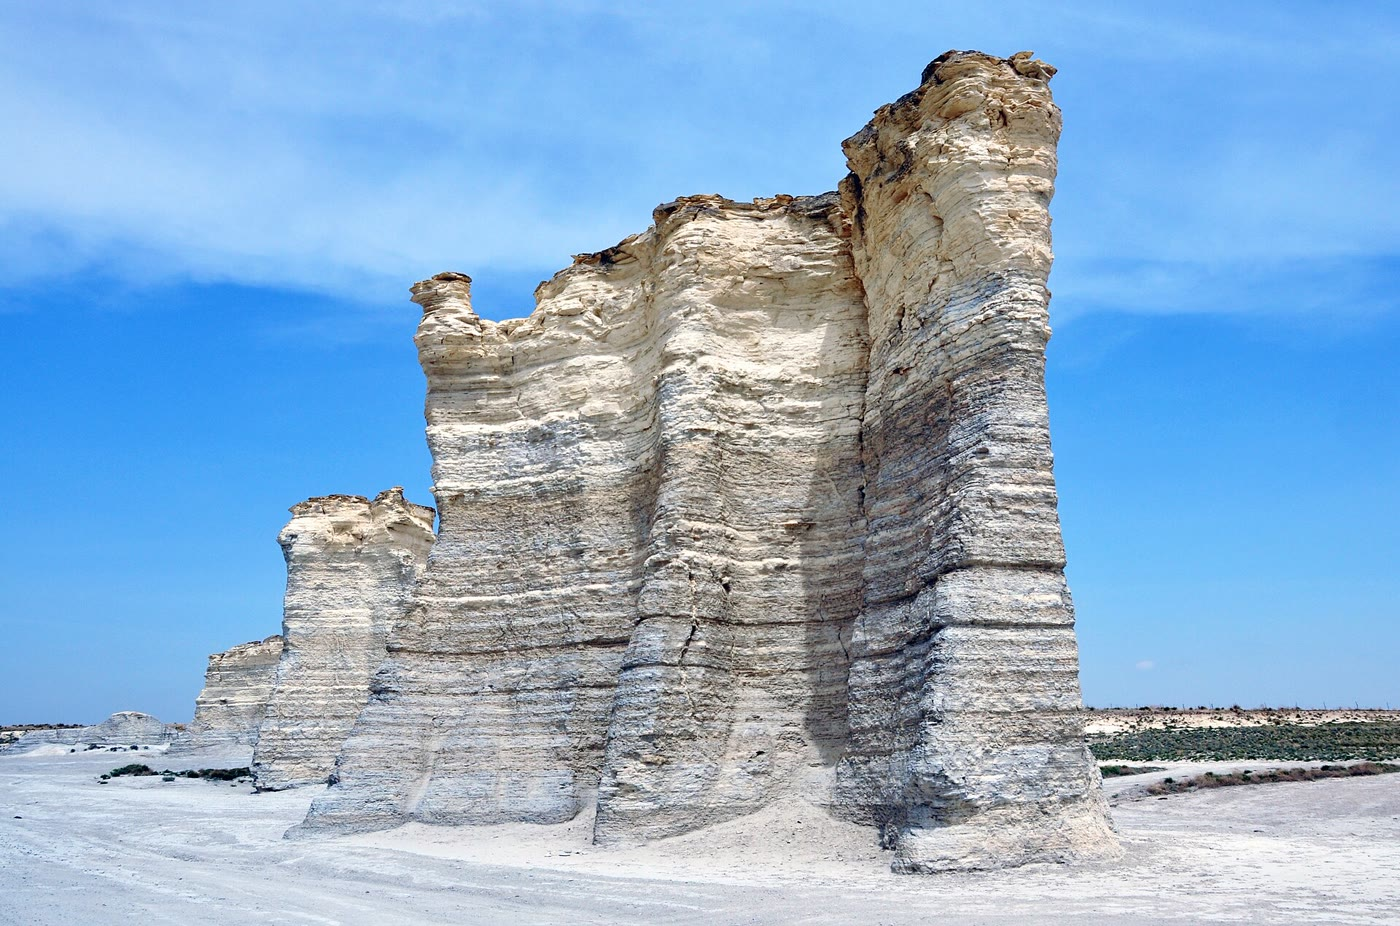
\includegraphics[width=0.66\linewidth]{images/book4/b2-19-monument-rocks.jpg}
\par\smallskip{\small Monument Rocks, oeste do Kansas: pilares de giz, a vasa de um mar interior
cretáceo de cerca de 80 milhões de anos, depositada a cerca de \qty{0.036}{mm} por ano. (Fotografia de James St.~John,
CC~BY~2.0, via Wikimedia Commons.)}
\end{omfigure}
% ledger: kgs:monument-rocks, kgs:chalk

\begin{definition}[Mar epicontinental]\label{def:b2:phanerozoic-earth:epeiric}
Um \emph{mar epicontinental}\index{mar epicontinental} (mar epírico) é um mar raso espalhado sobre o interior de um
continente, sobre crosta continental, longe da margem continental.
\end{definition}

O mar chega a esses interiores deslocando sua costa, e as rochas registram esse movimento.

\begin{definition}[Transgressão marinha; regressão marinha]\label{def:b2:phanerozoic-earth:transgression}
Uma \emph{transgressão marinha}\index{transgressão marinha} é um deslocamento da linha de costa em direção ao continente,
pelo qual o mar se espalha sobre a terra; uma \emph{regressão marinha}\index{regressão marinha} é
um deslocamento em direção ao mar, pelo qual a terra emerge.
\end{definition}

Numa seção vertical, uma transgressão empilha depósitos de águas mais profundas sobre outros mais rasos ---
lama de plataforma externa sobre areia de praia --- e uma regressão, o inverso. Ambas seguem o nível relativo do
mar, que mistura o nível global do mar com a subsidência ou o soerguimento do local e com o
aporte de sedimento: um delta pode empurrar sua costa mar adentro enquanto o mar sobe, se for alimentado depressa
o bastante. Para ler o nível global do mar nas transgressões, um geólogo deve encontrar o mesmo sinal
em vários continentes, ou remover a subsidência por \omterm{def:b2:basins-compared:backstripping}{backstripping}, como no
\cref{ch:b2:basins-compared}.
% ledger: miller20:rsl

\subsection*{A curva de longo prazo}

\begin{definition}[Ciclo de primeira ordem do nível do mar]\label{def:b2:phanerozoic-earth:first-order}
O \emph{ciclo de primeira ordem do nível do mar}\index{ciclo de primeira ordem do nível do mar} é a parte mais lenta
da variação do nível global do mar, em escalas de tempo de dezenas a centenas de milhões de anos, fixada pela
tectônica da Terra sólida e não pelo gelo.
\end{definition}

Ao longo do Fanerozoico a curva de primeira ordem tem a forma de um M: alta no início do Paleozoico,
baixa enquanto a Pangeia se montou e permaneceu, do Carbonífero ao fim do Triássico, alta
de novo no Cretáceo, e em queda desde então. Extrapolada a partir da América do Norte, a inundação do Ordoviciano
Superior sozinha sugere uma subida adicional de 100 a \qty{200}{m}.
Variações mais rápidas se sobrepõem a essa curva: as comandadas pelo gelo registram-se em escalas de tempo de $10^4$ a
$10^6$ anos, e o manto de gelo antártico, a partir de cerca de \qty{33.5}{Ma}, moveu o mar de 50 a
\qty{60}{m}.
% ledger: th23:flooding, miller11:greenhouse, miller05:abstract

\begin{omfigure}
\centering
% figdata/bachelor-2/phanerozoic.py parts sealevel-haq, sealevel-haqlt, sealevel-kominz, sealevel-kominzlt
\begin{tikzpicture}
\begin{axis}[width=0.92\linewidth, height=6.2cm, x dir=reverse, xmin=0, xmax=252,
  ymin=-130, ymax=280, xlabel={idade (\unit{Ma})}, ylabel={nível do mar acima do atual (\unit{m})},
  xtick={0,50,...,250}, ytick={-100,-50,...,250}, xtick pos=bottom, ytick pos=left,
  tick label style={font=\scriptsize}, label style={font=\small},
  legend style={at={(0.5,1.04)}, anchor=south, draw=none, font=\scriptsize, legend columns=2,
  /tikz/every even column/.append style={column sep=8pt}}]
\addplot[black!30, line width=0.3pt] table[x=age_ma, y=sl_m]
  {figdata/out/bachelor-2-phanerozoic-sealevel-haq.dat};
\addlegendentry{Haq e colaboradores (1987)}
\addplot[omThm, line width=0.3pt] table[x=age_ma, y=sl_m]
  {figdata/out/bachelor-2-phanerozoic-sealevel-kominz.dat};
\addlegendentry{Nova Jersey, com backstripping}
\addplot[black, line width=1.2pt] table[x=age_ma, y=sl_m]
  {figdata/out/bachelor-2-phanerozoic-sealevel-haqlt.dat};
\addlegendentry{Haq, média de 10 Myr}
\addplot[omThm!70!black, line width=1.2pt] table[x=age_ma, y=sl_m]
  {figdata/out/bachelor-2-phanerozoic-sealevel-kominzlt.dat};
\addlegendentry{Nova Jersey, média de 10 Myr}
\addplot[black!50, line width=0.3pt, forget plot] coordinates {(0,0) (252,0)};
\foreach \a/\b/\c in {251.902/201.4/icsTriassic, 201.4/143.1/icsJurassic,
  143.1/66/icsCretaceous, 66/23.04/icsPaleogene, 23.04/2.58/icsNeogene, 2.58/0/icsQuaternary} {
  \edef\tmp{\noexpand\fill[\c] (axis cs:\a,-130) rectangle (axis cs:\b,-112);}\tmp}
\node[font=\tiny, text=white] at (axis cs:226.7,-121) {Triássico};
\node[font=\tiny, text=white] at (axis cs:172.3,-121) {Jurássico};
\node[font=\tiny] at (axis cs:104.6,-121) {Cretáceo};
\node[font=\tiny] at (axis cs:44.5,-121) {Paleógeno};
\node[font=\tiny] at (axis cs:12.8,-121) {Neóg.};
\end{axis}
\end{tikzpicture}
\par\smallskip{\small O nível global do mar desde \qty{250}{Ma}, tal como tabulado por Miller e colaboradores
(2005): a carta de ciclos de Haq e colaboradores (1987), a partir da estratigrafia de muitas bacias, e o
nível do mar obtido por \omterm{def:b2:basins-compared:backstripping}{backstripping} de sondagens de Nova Jersey, com mínimos estimados (Kominz e
colaboradores 2008). Linhas grossas: médias móveis de 10 Myr, a tendência de primeira ordem. Idades na escala
de tempo de 2012; a barra embaixo mostra os períodos.}
\end{omfigure}
% ledger: data:b4-sealevel, haq87:charts, kominz08:long-term, ics:base.Triassic, ics:base.Jurassic, ics:base.Cretaceous, ics:base.Paleogene, ics:base.Neogene, ics:base.Quaternary, ics:colour.Triassic, ics:colour.Jurassic, ics:colour.Cretaceous, ics:colour.Paleogene, ics:colour.Neogene, ics:colour.Quaternary

As duas curvas acima concordam na forma e discordam no tamanho. A carta de ciclos, construída a partir
do empilhamento de sedimentos em muitas bacias, põe o nível do mar de longo prazo do Cretáceo médio
cerca de \qty{233}{m} acima do atual; os poços de Nova Jersey, submetidos a \omterm{def:b2:basins-compared:backstripping}{backstripping} um a um, dão cerca de
\qty{70}{m} no Cretáceo Superior e um máximo perto de \qty{110}{m} no Eoceno. Miller e seus
colegas concluem que o pico de longo prazo do Cretáceo foi de $100 \pm \qty{50}{m}$, e que as
cartas de ciclos, certas quanto à cronologia das quedas, exageram suas amplitudes. Mesmo Nova Jersey
não é um medidor perfeito: seu mar do Cretáceo Superior está de 100 a \qty{150}{m} abaixo do que o volume
das bacias oceânicas prevê, uma diferença que o afundamento da região acima da placa Farallon subductada
--- a topografia dinâmica --- poderia explicar.
% ledger: data:b4-sealevel, miller05:abstract, kominz08:long-term, miller20:epr

\subsection*{Por que o mar se move: as dorsais}

O que eleva o mar em uma centena de metros por dezenas de milhões de anos? Não o gelo: o Cretáceo
foi um mundo quente, com no máximo mantos de gelo pequenos e efêmeros. A principal resposta é o volume das
dorsais oceânicas. O fundo oceânico jovem é quente e fica alto; quanto mais depressa as placas se afastam, mais
jovem é o fundo em média, mais rasas as bacias oceânicas, e mais água transborda sobre
os continentes.
% ledger: miller11:greenhouse, th23:pitman

\begin{proposition}[Nível do mar e taxa de expansão]\label{prop:b2:phanerozoic-earth:ridge}
Seja um fundo oceânico de área $A_{\text{f}}$ produzido em dorsais de comprimento total $L$ à taxa de
expansão total $u$, e destruído na idade $\tau = A_{\text{f}}/(Lu)$, cada idade entre 0
e $\tau$ cobrindo a mesma área. Seja sua profundidade dada pela lei $d(t) = d_{\text{r}} + c\sqrt t$.
\begin{enumerate}
  \item A profundidade média do fundo é $\bar d = d_{\text{r}} + \tfrac23 c\sqrt\tau$.
  \item Se a taxa de expansão passa a $fu$, com $A_{\text{f}}$ e $L$ inalterados, a profundidade
        média diminui de $\Delta\bar d = \tfrac23 c\sqrt\tau\,\bigl(1 - f^{-1/2}\bigr)$.
  \item Se o fundo afunda isostaticamente sob a água acrescentada, e o mar não se espalha
        sobre a terra, o nível do mar sobre um oceano de área $A_{\text{o}}$ sobe de
        \[
        \Delta s = \frac{\rho_{\text{m}} - \rho_{\text{w}}}{\rho_{\text{m}}}\,
        \frac{A_{\text{f}}}{A_{\text{o}}}\,\Delta\bar d ,
        \]
        sendo $\rho_{\text{m}}$ a densidade do manto e $\rho_{\text{w}}$ a da água do mar.
\end{enumerate}
\end{proposition}

\begin{proof}
(1) As dorsais produzem fundo novo à taxa $Lu$ (área por unidade de tempo), e cada faixa de fundo vive
durante o tempo $\tau$; em regime estacionário a área de fundo com idade entre $t$ e $t + \mathrm{d}t$
é $Lu\,\mathrm{d}t$ para todo $t < \tau$, de modo que a área total é $Lu\tau = A_{\text{f}}$ e as
idades estão uniformemente distribuídas. A profundidade média é
$\frac1\tau\int_0^\tau (d_{\text{r}} + c\sqrt t)\,\mathrm{d}t = d_{\text{r}} + \frac{c}{\tau}
\cdot\frac23\tau^{3/2}$. (2) Com a taxa $fu$, $\tau$ passa a $\tau/f$, e
$\sqrt{\tau/f} = f^{-1/2}\sqrt\tau$. (3) As bacias perdem o volume $\Delta V = A_{\text{f}}
\Delta\bar d$. Suponha-se que a superfície do mar suba de $\Delta s$ em relação aos continentes, e que o fundo afunde
de $y$ sob a água extra. A coluna de água extra, de espessura $\Delta s + y$, substitui uma
espessura $y$ de manto no equilíbrio isostático: $\rho_{\text{w}}(\Delta s + y) =
\rho_{\text{m}} y$, logo $y = \rho_{\text{w}}\Delta s/(\rho_{\text{m}} - \rho_{\text{w}})$ e
$\Delta s + y = \Delta s\,\rho_{\text{m}}/(\rho_{\text{m}} - \rho_{\text{w}})$. O volume se
conserva: $A_{\text{o}}(\Delta s + y) = \Delta V$, o que dá o resultado.
\end{proof}

O fundo real não é tão ordenado. Suas idades não estão uniformemente distribuídas: o fundo jovem é o mais abundante,
e a área diminui com a idade, como mostra o painel esquerdo abaixo. Nem a lei da raiz quadrada vale para o
fundo antigo, que se aplaina perto de \qty{6.4}{km}; a lei exponencial que Parsons e Sclater
ajustaram ao fundo antigo, a lei da placa, assume além de cerca de \qty{26}{Myr}, onde as duas leis
se encontram. A proposição é uma primeira estimativa, e a figura
mostra quanto a segunda lei a altera.
% ledger: ps77:depth-age, data:b4-ridge

\begin{omfigure}
\centering
% figdata/bachelor-2/phanerozoic.py parts agehist and ridge
\begin{tikzpicture}
\begin{groupplot}[group style={group size=2 by 1, horizontal sep=1.6cm},
  width=0.5\linewidth, height=5.6cm, tick label style={font=\scriptsize},
  label style={font=\small}, xtick pos=bottom, ytick pos=left]
\nextgroupplot[xmin=0, xmax=200, ymin=0, ymax=34, xlabel={idade do fundo (\unit{Myr})},
  ylabel={área por \qty{10}{Myr} (\unit{\mega km^2})},
  legend style={at={(0.5,1.04)}, anchor=south, draw=none, font=\scriptsize}]
\addplot[ybar interval, area legend, fill=omSea!80!black, draw=black!50, line width=0.2pt]
  table[x expr=\thisrow{age}-5, y=area_Mkm2] {figdata/out/bachelor-2-phanerozoic-agehist.dat};
\addlegendentry{grade de idades}
\addplot[const plot mark mid, black, dashed, line width=0.9pt]
  table[x=age, y=uniform_Mkm2] {figdata/out/bachelor-2-phanerozoic-agehist.dat};
\addlegendentry{idades uniformes até \qty{128.4}{Myr}}
\nextgroupplot[xmin=1, xmax=3, ymin=0, ymax=650, xlabel={taxa de expansão / atual, $f$},
  ylabel={subida do nível do mar $\Delta s$ (\unit{m})},
  legend style={at={(0.5,1.04)}, anchor=south, draw=none, font=\scriptsize, legend columns=2}]
\fill[omThm!15] (axis cs:1,50) rectangle (axis cs:3,150);
\addplot[black, line width=1pt] table[x=f, y=ds_hs] {figdata/out/bachelor-2-phanerozoic-ridge.dat};
\addlegendentry{lei em $\sqrt t$}
\addplot[blue!70!black, dashed, line width=1pt] table[x=f, y=ds_plate]
  {figdata/out/bachelor-2-phanerozoic-ridge.dat};
\addlegendentry{lei da placa}
\node[font=\scriptsize, anchor=west] at (axis cs:1.6,100) {$100 \pm \qty{50}{m}$};
\end{groupplot}
\end{tikzpicture}
\par\smallskip{\small Esquerda: área do fundo oceânico atual em classes de idade de 10 Myr, a partir da grade de idades
de Seton e colaboradores (2020) com resolução de um grau (\qty{293}{\mega km^2} no total), contra a
distribuição uniforme da \cref{prop:b2:phanerozoic-earth:ridge} com a mesma área e a mesma idade média. Direita:
subida do nível do mar quando a taxa de expansão é multiplicada por $f$, pela proposição com a
lei da raiz quadrada e com a lei da placa, partindo da distribuição uniforme até \qty{128.4}{Myr}; a
faixa é o pico de longo prazo do Cretáceo estimado por Miller e colaboradores (2005).}
\end{omfigure}
% ledger: data:b4-ridge, data:b2-seafloor-age, seton:mean-age, ps77:depth-age, miller05:abstract, charette:ocean-volume, katz03:thermo, noaa:seawater-1025

\begin{example}[Duas vezes mais rápido]\label{ex:b2:phanerozoic-earth:doubling}
Tome-se o fundo atual: idade média \qty{64.2}{Myr}, logo $\tau = \qty{128.4}{Myr}$ no modelo uniforme;
$d_{\text{r}} = \qty{2500}{m}$, $c = \qty{350}{m.Myr^{-1/2}}$. A profundidade média é $2500 + \tfrac23
\times 350 \times \sqrt{128.4} = \qty{5144}{m}$. Dobrar a taxa reduz $\tau$ à metade, e a profundidade
média passa a $2500 + \tfrac23 \times 350 \times \sqrt{64.2} = \qty{4370}{m}$: o fundo sobe
\qty{774}{m} em média. Com $A_{\text{f}}/A_{\text{o}} = 293/362 = 0.8094$ e
$(\rho_{\text{m}} - \rho_{\text{w}})/\rho_{\text{m}} = (3300 - 1025)/3300 = 0.689$, o mar sobe
$0.689 \times 0.8094 \times 774 = \qty{432}{m}$; com a lei da placa, \qty{368}{m}. Ambos são
cerca de quatro vezes o pico de longo prazo do Cretáceo. Lido ao contrário, o painel direito diz que uma
taxa de expansão apenas 15 a \qty{20}{\percent} acima da atual basta para \qty{100}{m} --- e é
por isso que Miller e seus colegas concluem que a crosta oceânica foi produzida muito mais devagar no
Cretáceo do que se inferia antes.
\end{example}
% ledger: seton:mean-age, ps77:depth-age, data:b4-ridge, charette:ocean-volume, katz03:thermo, noaa:seawater-1025, miller05:abstract
% values (phanerozoic.py numbers): dbar_hs 5144, dbar_hs_half 4369.6, rise2_hs 432.5, rise2_pl 368.4, f_for_100_hs 1.151

O modelo também é profundo demais: sua profundidade média, \qty{5144}{m}, excede a profundidade média medida
do fundo datado, \qty{4265}{m}, em parte porque a lei da raiz quadrada exagera no fundo antigo, e
em parte porque o fundo real carrega sedimento, \omterm{def:b2:oceanic-islands:seamount}{montes submarinos} e platôs que a lei deixa de fora. E a expansão não é a
única alavanca. As dorsais são compensadas pelas fossas: se o fundo oceânico sobe num lugar, a massa tem de
ir para algum lugar, e um continente que afunda sobre uma placa subductada --- a topografia dinâmica --- deixa o mar entrar
localmente. Tasistro-Hart e Macdonald argumentam que as inundações da América do Norte seguem as placas subductadas
sob o continente, e que o nível global do mar depende de quanto da subducção ocorre sob
continentes e não sob oceanos.
% ledger: data:b4-floor-depth, th23:pitman, th23:flooding, kominz08:long-term

\section{A inundação dos continentes}\label{sec:b2:phanerozoic-earth:flooding}

Quanta terra uma subida do mar afoga depende da forma da superfície da Terra, que a
curva hipsométrica do volume do primeiro ano resume: a fração da superfície que fica acima de
cada altitude (figura abaixo, à esquerda). Os continentes têm o topo plano. Na grade de um grau do
ETOPO1, \qty{29.0}{\percent} da superfície é terra e \qty{34.3}{\percent} fica acima de
\qty{-200}{m}: as plataformas, já sob a água, fazem a diferença. A maior parte da terra é baixa, de modo que uma
subida modesta inunda uma grande parte dela.
% ledger: data:b4-hyps, data:etopo1

\begin{proposition}[A inundação da terra]\label{prop:b2:phanerozoic-earth:flooding}
Seja $A_{\text{o}}$ a área do mar hoje e $a(z)$ a área de terra mais baixa que $z$ acima
do nível do mar atual. Um volume $V$ de água acrescentado ao mar eleva seu nível da altura $s$
que resolve
\[
V = \int_0^s \bigl(A_{\text{o}} + a(z)\bigr)\,\mathrm{d}z ,
\]
e inunda a área de terra $a(s)$. Como $a \ge 0$, a subida é no máximo $V/A_{\text{o}}$.
\end{proposition}

\begin{proof}
Quando o mar está em $z$, ele cobre $A_{\text{o}} + a(z)$; elevá-lo de $\mathrm{d}z$ exige
o volume $\bigl(A_{\text{o}} + a(z)\bigr)\mathrm{d}z$. Somando de 0 a $s$ obtém-se $V$. O
integrando é pelo menos $A_{\text{o}}$, de modo que $V \ge A_{\text{o}}s$.
\end{proof}

\begin{omfigure}
\centering
% figdata/bachelor-2/phanerozoic.py parts hyps and flood
\begin{tikzpicture}
\begin{groupplot}[group style={group size=2 by 1, horizontal sep=1.6cm},
  width=0.46\linewidth, height=5.6cm, tick label style={font=\scriptsize},
  label style={font=\small}, xtick pos=bottom, ytick pos=left]
\nextgroupplot[xmin=0, xmax=100, ymin=-9500, ymax=6500,
  xlabel={porcentagem da superfície acima de $z$}, ylabel={altitude $z$ (\unit{m})},
  scaled y ticks=false, yticklabel style={/pgf/number format/1000 sep={\,}}]
\addplot[omThm, line width=1pt] table[x=pct, y=z] {figdata/out/bachelor-2-phanerozoic-hyps.dat};
\addplot[black!50, line width=0.3pt] coordinates {(0,0) (100,0)};
\node[font=\scriptsize, anchor=south west] at (axis cs:30,100) {terra \qty{29.0}{\percent}};
\node[font=\scriptsize] at (axis cs:45,-7000) {fundo oceânico};
\nextgroupplot[xmin=0, xmax=1000, ymin=0, ymax=80, xlabel={subida do nível do mar $h$ (\unit{m})},
  ylabel={terra inundada (\unit{\percent})}]
\addplot[omThm, line width=1pt] table[x=h, y=flooded_pct]
  {figdata/out/bachelor-2-phanerozoic-flood.dat};
\addplot[black, dashed, line width=0.5pt] coordinates {(100,0) (100,14.9) (0,14.9)};
\addplot[black, dashed, line width=0.5pt] coordinates {(432,0) (432,50.6) (0,50.6)};
\end{groupplot}
\end{tikzpicture}
\par\smallskip{\small Esquerda: curva hipsométrica da Terra a partir da grade ETOPO1 de um grau.
Direita: porcentagem da terra atual abaixo de cada altura acima do nível do mar, a terra que uma subida $h$
inundaria se nada mais se movesse; as linhas tracejadas marcam \qty{100}{m} e \qty{432}{m}. A média sobre
células de um grau suaviza o relevo, de modo que estas são primeiras estimativas.}
\end{omfigure}
% ledger: data:b4-hyps, data:etopo1

O painel direito dá a resposta de imediato. Uma subida de \qty{100}{m} afoga cerca de
\qty{15}{\percent} da terra atual; os \qty{432}{m} de uma taxa de expansão dobrada afogariam
metade. Um mar assim se espalha sobre a terra que inunda, de modo que a própria subida é menor que o
limite $V/A_{\text{o}}$ da proposição, em cerca de um décimo para uma subida de algumas centenas de metros (problema de
fim de semana). Os mares cretáceos do Kansas precisaram de muito menos: o interior de um continente é muitas vezes
baixo, e pode também afundar sobre uma placa subductada.
% ledger: data:b4-hyps
% values (phanerozoic.py numbers): flood_100 14.9, flood_rise2 50.8, level_rise2_spread 390.7

\section{Cadeias de montanhas do Fanerozoico}\label{sec:b2:phanerozoic-earth:orogens}

Cada \omterm{def:b2:wilson-cycle:wilson}{ciclo de Wilson} do \cref{ch:b2:wilson-cycle} termina numa cadeia de montanhas, e as cadeias
fanerozoicas marcam a montagem e a fragmentação da Pangeia. A tabela reúne as encontradas neste volume.

\begin{center}
\small
\begin{tabular}{>{\raggedright\arraybackslash}p{0.15\linewidth}>{\raggedright\arraybackslash}p{0.22\linewidth}>{\raggedright\arraybackslash}p{0.22\linewidth}>{\raggedright\arraybackslash}p{0.29\linewidth}}
\hline
orogenia & época & oceano fechado & o que colidiu \\
\hline
Caledoniana & c.~540--400 Ma; colisão principal 425--400 Ma & Iapetus & Laurentia, Báltica e
Avalônia, formando a Laurússia \\
Varisca--apalachiana & desde c.~550 Ma; colisão final Carbonífero Superior--Permiano & Rheic &
o Gondwana e seus terrenos destacados com a Laurússia, formando a Pangeia \\
Alpina & Cretáceo (pico perto de 100 Ma) e Cenozoico & Tétis Alpino & Apúlia e Europa \\
Himalaiana & desde c.~60 a 54 Ma (debatido) até hoje & oceano ao norte da Índia & Índia e Ásia \\
Andina & ainda ativa; encurtamento desde o Oligoceno & nenhum: uma placa oceânica é subductada & a
placa de Nazca sob a América do Sul \\
\hline
\end{tabular}
\end{center}
% ledger: mckerrow00:caledonian, schiffer20:caledonides, schiffer20:variscan, faure24:variscan, usgs:alleghanian-age, schmid04:two-orogenies, najman21:collision-age, gerbault05:andes, nance22:supercontinents

As duas primeiras cadeias costuraram a Pangeia, a varisca fechando o último oceano entre o Gondwana
e a Laurússia; as três últimas cresceram à medida que os pedaços da Pangeia se afastavam e os oceanos entre
eles eram consumidos. O nível do mar baixo do fim do Paleozoico e do Triássico pertence a esse
\omterm{def:b2:wilson-cycle:supercontinent}{supercontinente}, e o mar alto do Cretáceo à sua fragmentação, com novas dorsais e
fundo jovem.
% ledger: schiffer20:variscan, th23:flooding, nance22:supercontinents

\section{Crises da vida}\label{sec:b2:phanerozoic-earth:extinctions}

\subsection*{As cinco grandes}

Os volumes de biologia descrevem as extinções em massa; os geólogos as medem nas rochas e procuram
suas causas. Cinco se destacam no registro dos animais marinhos, as ``cinco grandes'': no fim do
Ordoviciano, há cerca de \qty{444}{Ma}; no Devoniano Superior, \qty{372}{Ma}; no fim do Permiano,
\qty{251.9}{Ma}; no fim do Triássico, \qty{201.4}{Ma}; e no fim do Cretáceo,
\qty{66}{Ma}. Cada uma eliminou entre cerca de dois quintos e dois terços dos gêneros de animais
marinhos na compilação de Sepkoski. A crise do fim do Permiano foi a maior: \qty{56}{\percent} dos
gêneros na resolução mais fina, e cerca de \qty{81}{\percent} das espécies marinhas --- não os
\qty{96}{\percent} muitas vezes citados, que misturavam duas crises distintas.
% ledger: kaiho22:table, marshall23:big-five, stanley16:permian

\begin{history}[As cinco grandes, quarenta anos depois]
Em 1982, D.~M.~Raup e J.~J.~Sepkoski contaram as famílias de animais marinhos que desapareceram
em cada um dos 76 andares do Fanerozoico. Quatro pontos ficaram acima do limite de confiança de 99~por cento
de sua tendência --- o último andar do Ordoviciano, os dois últimos do Permiano e o último do
Cretáceo --- e o fim do Triássico e o fim do Devoniano acima do limite de 95~por cento:
as cinco grandes. Quarenta anos depois, as cinco continuam sendo as maiores crises desde o início do
Ordoviciano, mas, com dados melhores, já não se destacam de um contínuo de taxas de
extinção, e alguns intervalos do Cambriano tiveram taxas até mais altas. A resolução temporal de Raup e Sepkoski
era de \qty{7.4}{Myr}, a duração média de um andar na época; algumas crises foram súbitas, outras
duraram centenas de milhares de anos ou mais.
\end{history}
% ledger: marshall23:big-five, marshall23:resolution

\begin{omfigure}
\centering
% figdata/bachelor-2/phanerozoic.py parts ext, lip, oae
\begin{tikzpicture}
\begin{axis}[width=0.95\linewidth, height=6.4cm, x dir=reverse, xmin=0, xmax=541,
  ymin=-34, ymax=80, xlabel={idade (\unit{Ma})}, ylabel={gêneros marinhos perdidos (\unit{\percent})},
  xtick={0,100,...,500}, ytick={0,20,...,80}, xtick pos=bottom, ytick pos=left,
  tick label style={font=\scriptsize}, label style={font=\small}, clip=false]
\addplot[ybar, bar width=5pt, fill=omThm!70, draw=black!60]
  % rótulos: nós explícitos (a tabela figdata traz os nomes em inglês)
  table[x=age, y=value] {figdata/out/bachelor-2-phanerozoic-ext.dat}; \foreach \a/\v/\t in {444/52/fim do Ordoviciano, 372/41/Devoniano Superior, 251.9/66/fim do Permiano, 201.4/46/fim do Triássico, 66/45/fim do Cretáceo} {\edef\temp{\noexpand\node[font=\noexpand\tiny, anchor=south] at (axis cs:\a,\v) {\t};}\temp}
\addplot[only marks, mark=triangle*, mark size=2.6pt, red!70!black]
  table[x=age, y expr=-6] {figdata/out/bachelor-2-phanerozoic-lip.dat};
\addplot[only marks, mark=diamond*, mark size=2.6pt, blue!70!black]
  table[x=age, y expr=-13] {figdata/out/bachelor-2-phanerozoic-oae.dat};
\addplot[only marks, mark=star, mark size=4pt, line width=1pt, black] coordinates {(66,-20)};
\node[font=\tiny, anchor=west, red!70!black] at (axis cs:541,-6) {GPIs};
\node[font=\tiny, anchor=west, blue!70!black] at (axis cs:541,-13) {OAEs};
\node[font=\tiny, anchor=west] at (axis cs:541,-20) {impacto};
\node[font=\tiny, anchor=west] at (axis cs:57,-20) {Chicxulub};
\foreach \a/\b/\c in {538.8/486.85/icsCambrian, 486.85/443.1/icsOrdovician,
  443.1/419.62/icsSilurian, 419.62/358.86/icsDevonian, 358.86/298.9/icsCarboniferous,
  298.9/251.902/icsPermian, 251.902/201.4/icsTriassic, 201.4/143.1/icsJurassic,
  143.1/66/icsCretaceous, 66/23.04/icsPaleogene, 23.04/2.58/icsNeogene, 2.58/0/icsQuaternary} {
  \edef\tmp{\noexpand\fill[\c] (axis cs:\a,-34) rectangle (axis cs:\b,-27);}\tmp}
\foreach \x/\t in {512.8/Cm, 465/O, 431.4/S, 389.2/D, 328.9/C, 275.4/P, 226.7/Tr, 172.3/J,
  104.6/K, 44.5/Pg, 12.8/N} {
  \edef\tmp{\noexpand\node[font=\noexpand\tiny] at (axis cs:\x,-30.5) {\t};}\tmp}
\end{axis}
\end{tikzpicture}
\par\smallskip{\small As cinco grandes extinções em massa, com a parcela de gêneros marinhos perdidos na
compilação de Sepkoski (Kaiho 2022, Tabela~1), as grandes províncias ígneas (GPIs; triângulos, idades médias de
Courtillot e Renne 2003, a partir de \qty{259}{Ma}), os \omterm{def:b2:phanerozoic-earth:oae}{eventos anóxicos oceânicos} (OAE) mais estudados
(losangos) e o impacto de Chicxulub. A barra embaixo mostra os períodos.}
\end{omfigure}
% ledger: kaiho22:table, cr03:table, rigo24:oaes, pickersgill26:chicxulub, ics:base.Cambrian, ics:base.Ordovician, ics:base.Silurian, ics:base.Devonian, ics:base.Carboniferous, ics:base.Permian, ics:base.Triassic, ics:base.Jurassic, ics:base.Cretaceous, ics:base.Paleogene, ics:base.Neogene, ics:base.Quaternary, ics:colour.Cambrian, ics:colour.Ordovician, ics:colour.Silurian, ics:colour.Devonian, ics:colour.Carboniferous, ics:colour.Permian

\subsection*{Grandes províncias ígneas}

A figura acima mostra o padrão que o volume do primeiro ano apontou: as três mais recentes das
cinco grandes coincidem cada uma com uma grande província ígnea, os Traps Siberianos no fim do Permiano,
a Província Magmática do Atlântico Central (CAMP) no fim do Triássico, os Traps do Decã no
fim do Cretáceo. O vínculo proposto é o gás. Um basalto de platô extravasa em pulsos de alguns
séculos a alguns milênios, cada um liberando dióxido de carbono mais depressa do que o intemperismo consegue
retirá-lo; o enxofre das mesmas erupções resfria o clima brevemente, o carbono o aquece por muito
mais tempo e acidifica o oceano.
% ledger: cr03:table, cr03:summary, capriolo20:camp-co2

\begin{example}[O carbono da província do Atlântico Central]\label{ex:b2:phanerozoic-earth:camp}
Bolhas de gás em inclusões de fundido de basaltos da CAMP mostram que o \omterm{def:b2:magma-emplacement:magma}{magma} continha pelo menos 0.5 a
\qty{0.6}{\percent} de dióxido de carbono em massa. Tome-se \qty{0.55}{\percent}, uma densidade de
\qty{2900}{kg.m^{-3}} e um volume de \qty{5.5e6}{km^3}, as lavas extravasadas com os \omterm{def:b2:magma-emplacement:bodies}{diques}, as \omterm{def:b2:magma-emplacement:bodies}{soleiras}
e as câmaras que as alimentaram. A massa de \omterm{def:b2:magma-emplacement:magma}{magma} é $\num{5.5e6} \times \num{e9} \times 2900 =
\qty{1.6e19}{kg}$, e seu dióxido de carbono $\num{1.6e19} \times 0.0055 = \qty{8.8e16}{kg}$, cerca de
\qty{9e4}{Gt} --- o ``até \qty{e5}{Gt}'' dos autores. Liberado ao longo da vida da província, ele
não esteve todo no ar ao mesmo tempo; mas cada pulso, da ordem de \qty{e5}{km^3} em alguns
séculos, liberou tanto quanto as emissões projetadas para o século XXI.
\end{example}
% ledger: capriolo20:camp-co2
% values: 5.5e6 km3 x 2900 kg/m3 = 1.595e19 kg; x 0.0055 = 8.77e16 kg

\subsection*{Eventos anóxicos oceânicos}

Nem toda crise é uma das cinco grandes. Várias vezes no Mesozoico, o oxigênio desapareceu de
grandes partes do oceano.

\begin{definition}[Evento anóxico oceânico]\label{def:b2:phanerozoic-earth:oae}
Um \emph{evento anóxico oceânico}\index{evento anóxico oceânico} (OAE) é um intervalo de
depleção generalizada de oxigênio no oceano, reconhecido no registro sedimentar e geoquímico.
\end{definition}

Sua marca habitual é um folhelho negro: escuro, finamente laminado, sem bioturbação, rico em matéria orgânica
e em pirita, muitas vezes com um desvio dos isótopos de carbono e sinais de aquecimento. Os mais bem estudados
são o evento do Toarciano inferior, há cerca de \qty{183}{Ma}, o OAE~1a do Aptiano inferior, há cerca de \qty{120}{Ma},
o OAE~1b do Albiano inferior, há cerca de \qty{111}{Ma}, e o OAE~2 no limite entre o Cenomaniano
e o Turoniano, há cerca de \qty{94}{Ma}, na parte mais quente do Cretáceo, quando o mar estava
excepcionalmente alto. Vários coincidem com uma província: o evento do Toarciano com os basaltos de Karoo--Ferrar,
o OAE~1a com o platô de Ontong Java. O OAE~2 é muitas vezes ligado ao platô do Caribe, mas
picos de mercúrio em sedimentos do Hemisfério Sul apontam, em vez disso, para a província de Kerguelen.
% ledger: rigo24:oaes, wt24:oae2, cr03:table

\begin{omfigure}
\centering
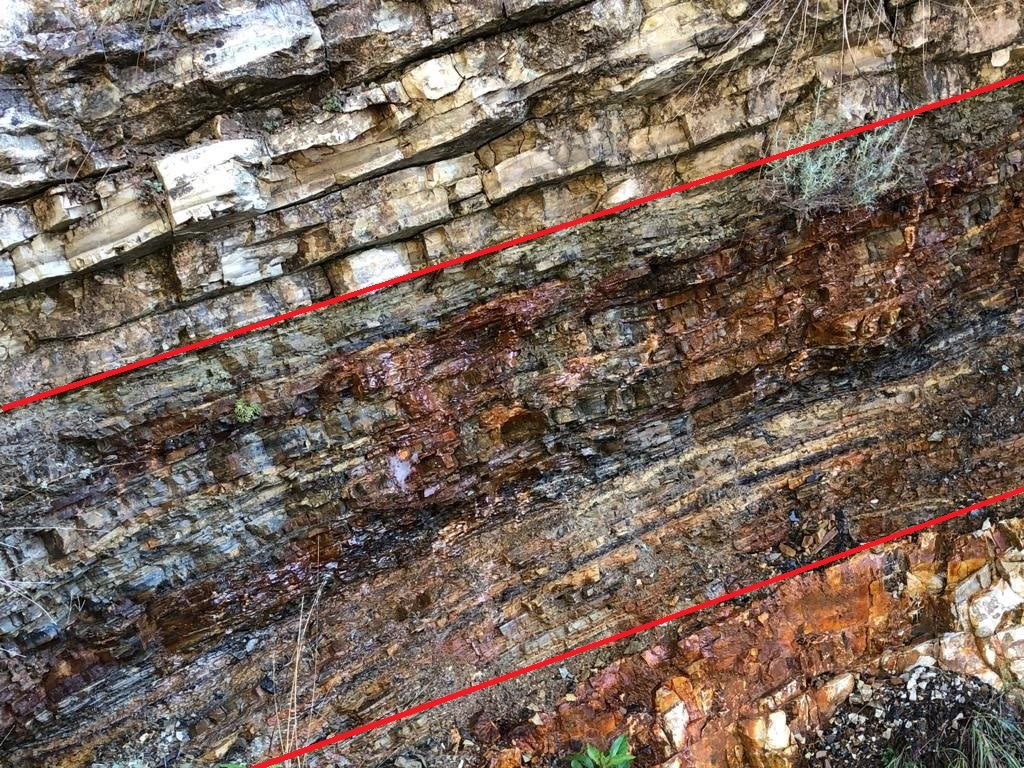
\includegraphics[width=0.66\linewidth]{images/book4/b2-19-bonarelli-level.jpg}
\par\smallskip{\small O nível Bonarelli, o folhelho escuro do OAE~2, entre calcários claros; as
linhas vermelhas, traçadas pelo fotógrafo, marcam sua base e seu topo. (Picenus, CC~BY-SA~4.0, via
Wikimedia Commons.)}
\end{omfigure}
% ledger: rigo24:oaes

\begin{inthefield}[Registrar um evento anóxico]
Uma geóloga que estuda um OAE numa seção de calcários pelágicos registra-o camada por camada: espessura,
cor, laminação, bioturbações ou sua ausência, nódulos de pirita. Ela amostra a intervalos curtos e regulares
através do intervalo escuro e bem além dele, para o teor de carbono orgânico e para os
isótopos de carbono da matéria orgânica e do carbonato; o desvio dos isótopos, mais do que
a cor da rocha, correlaciona o evento de uma bacia para a outra. Como o folhelho mais escuro
pode aparecer em níveis diferentes em bacias diferentes, é a curva isotópica, e não o folhelho
negro, que se toma como linha de tempo.
\end{inthefield}
% ledger: rigo24:oaes, wt24:oae2

\subsection*{Chicxulub}

O fim do Cretáceo teve uma causa vinda de fora. O volume do primeiro ano contou como o irídio da
argila do limite levou a um impacto, e como a datação pelo argônio ligou o limite à cratera de Chicxulub.
A estrutura tem cerca de \qty{200}{km} de diâmetro e \qty{66}{Ma}; suas
rochas quentes alimentaram a circulação de água durante pelo menos oito milhões de anos depois. Modelos de sua assimetria
em subsuperfície apontam para um impactor vindo do nordeste a 45 a \ang{60} da horizontal,
a não menos que a velocidade de escape da Terra, \qty{11.2}{km.s^{-1}}, e mais provavelmente a cerca de
\qty{20}{km.s^{-1}}. Os Traps do Decã estavam em erupção ao mesmo tempo, antes e depois do
impacto; uma revisão das evidências em 2010 concluiu que o impacto desencadeou a extinção.
% ledger: pickersgill26:chicxulub, collins20:impact, renne:kpg, alvarez:iridium, schulte:kpg, cr03:deccan

\begin{dated}{2026}
As idades deste capítulo são as da Carta Cronoestratigráfica Internacional em sua versão de junho
de 2026, como em toda esta série; os registros do nível do mar estão na escala de tempo de 2012
de seus arquivos, e as idades das extinções são as de Kaiho (2022). A carta é revista à medida que chegam
novas datas: consulte a versão atual antes de citar a idade de um limite.
\end{dated}
% ledger: ics:base.Phanerozoic, data:b4-sealevel, kaiho22:table

\section*{Exercícios}\label{sec:b2:phanerozoic-earth:exercises}

Dados para os exercícios, salvo indicação em contrário: \qty{111.2}{km} por grau de latitude; profundidade
do fundo oceânico $d(t) = 2500 + 350\sqrt t$ (\unit{m}, $t$ em \unit{Myr}); área do oceano
\qty{362}{\mega km^2}; área do fundo oceânico \qty{293}{\mega km^2}; densidade do manto
\qty{3300}{kg.m^{-3}}; água do mar \qty{1025}{kg.m^{-3}}; massa da atmosfera
\qty{5.1e18}{kg}, massas molares do ar e do dióxido de carbono \qty{28.97}{g.mol^{-1}} e
\qty{44.01}{g.mol^{-1}}.
% ledger: earth:Rmean, ps77:depth-age, charette:ocean-volume, data:b4-ridge, katz03:thermo, noaa:seawater-1025, earth:Matm, earth:Mmol, ciaaw:abridged-2024

\begin{exercise}[$\star$]\label{exo:b2:phanerozoic-earth:1}
No modelo dos mapas, a Cidade do Cabo estava a \ang{61.9}~S há \qty{300}{Ma} e Nova York a
\ang{3.6}~S; hoje estão a \ang{33.9}~S e \ang{40.7}~N. (a) Quais das quatro cidades estavam
a menos de \ang{30} do equador há \qty{300}{Ma} (Paris a \ang{5.1}~N, Sydney a
\ang{59.5}~S)? (b) Quantos quilômetros para o norte se deslocaram desde então a Cidade do Cabo e Nova York?
(c) A que taxas médias, em centímetros por ano?
\end{exercise}
% ledger: data:b4-palaeopos, geonames4:cities

\begin{exercise}[$\star$]\label{exo:b2:phanerozoic-earth:2}
As cinco grandes ocorreram a 444, 372, 251.9, 201.4 e \qty{66}{Ma}. (a) Calcule os intervalos entre
crises sucessivas e sua média. (b) Usando as idades médias das grandes províncias ígneas ---
Emeishan 259, Sibéria 250, CAMP 201, Karoo--Ferrar 183, Decã \qty{65.5}{Ma} --- quais das
cinco caem a menos de \qty{2}{Myr} de uma província? (c) Um intervalo médio torna as crises periódicas?
\end{exercise}
% ledger: kaiho22:table, cr03:table

\begin{exercise}[$\star$]\label{exo:b2:phanerozoic-earth:3}
O giz de Monument Rocks depositou-se a cerca de \qty{0.036}{mm} por ano. (a) Quanto tempo levaram
\qty{91}{m} dele? (b) Quantas vezes mais depressa sobe o mar hoje, a \qty{3.7}{mm} por
ano? (c) Por que um fundo marinho pode recolher uma chuva tão lenta de sedimento sem ser soterrado por lama?
\end{exercise}
% ledger: kgs:monument-rocks, ipcc:sea-level-obs

\begin{exercise}[$\star$]\label{exo:b2:phanerozoic-earth:4}
Numa falésia, de baixo para cima: arenito fluvial com raízes, areia de praia com conchas, lama cinzenta
de plataforma externa, giz; depois o giz é recoberto de novo por areia de praia. (a) Onde a seção registra uma
\omterm{def:b2:phanerozoic-earth:transgression}{transgressão marinha}, e onde uma regressão? (b) A transgressão prova que o nível global do mar
subiu? (c) O que a tornaria mais convincente?
\end{exercise}

\begin{exercise}[$\star\star$]\label{exo:b2:phanerozoic-earth:5}
Na curva de longo prazo de Haq e colaboradores, o nível do mar estava \qty{233}{m} acima do atual a
\qty{97}{Ma}. (a) Que taxa média de queda desde então, em metros por milhão de anos e em
micrômetros por ano? (b) Compare com a subida atual de \qty{3.7}{mm} por ano. (c) A curva de Nova Jersey
obtida por \omterm{def:b2:basins-compared:backstripping}{backstripping} dá cerca de \qty{70}{m} na mesma época. Em qual você confiaria para a
amplitude, e por quê?
\end{exercise}
% ledger: data:b4-sealevel, ipcc:sea-level-obs, miller05:abstract, miller20:epr

\begin{exercise}[$\star\star$]\label{exo:b2:phanerozoic-earth:6}
Um único pulso da CAMP, cerca de \qty{e5}{km^3} de basalto de densidade \qty{2900}{kg.m^{-3}},
extravasou em cerca de 500 anos. (a) Com \qty{0.75}{\percent} de dióxido de carbono em massa, quanto
ele liberou, em quilogramas e em mols? (b) Que massa de dióxido de carbono o ar continha
às \qty{278}{ppm} de 1750? (c) Compare. (d) Quantas dessas atmosferas a província inteira,
\qty{e5}{Gt}, teria fornecido?
\end{exercise}
% ledger: capriolo20:camp-co2, ipcc:erf-2xco2, earth:Matm, earth:Mmol, ciaaw:abridged-2024

\begin{exercise}[$\star\star$]\label{exo:b2:phanerozoic-earth:7}
Tome o impactor de Chicxulub como uma esfera de \qty{10}{km} de diâmetro, de densidade
\qty{2630}{kg.m^{-3}}. (a) Calcule sua massa. (b) Calcule sua energia cinética à menor velocidade
possível, \qty{11.2}{km.s^{-1}}, e a \qty{20}{km.s^{-1}}. (c) A Terra perde \qty{47}{TW} de
calor interno por sua superfície. Quantos anos dessa perda cada energia representa?
\end{exercise}
% ledger: alvarez:iridium, collins20:impact, b2dd10:half-space

\begin{exercise}[$\star\star$]\label{exo:b2:phanerozoic-earth:8}
(a) Liste as características pelas quais um folhelho negro registra um \omterm{def:b2:phanerozoic-earth:oae}{evento anóxico oceânico}. (b) Associe cada
evento a uma província de quase a mesma idade: Toarciano inferior, \qty{183}{Ma}; OAE~1a,
\qty{120}{Ma}; dados Karoo--Ferrar a \qty{183}{Ma} e Ontong Java a \qty{122}{Ma}. (c) Por que uma
coincidência de idades não basta para provar que uma província causou um evento?
\end{exercise}
% ledger: rigo24:oaes, cr03:table

\begin{exercise}[$\star\star$]\label{exo:b2:phanerozoic-earth:9}
No modelo, Paris estava a \ang{60.9}~S há \qty{500}{Ma} e a \ang{5.1}~N há \qty{300}{Ma}.
(a) Calcule seu deslocamento para o norte em graus e em quilômetros, e a taxa média em
centímetros por ano. (b) Compare com a taxa desde \qty{300}{Ma}
(\cref{ex:b2:phanerozoic-earth:paris}). (c) Por que a taxa é um mínimo?
\end{exercise}
% ledger: data:b4-palaeopos

\begin{exercise}[$\star\star\star$]\label{exo:b2:phanerozoic-earth:10}
Suponha, em vez disso, que a área do fundo diminui linearmente com a idade, de um máximo na idade 0 a zero
na idade $T$. (a) Mostre que a idade média é $T/3$ e que a média de $\sqrt t$ é
$\tfrac{8}{15}\sqrt T$. (b) Com uma idade média de \qty{64.2}{Myr}, calcule $T$ e a profundidade média. (c)
Calcule a queda da profundidade média quando a taxa de expansão dobra, e compare com os
\qty{774}{m} do modelo uniforme. (d) Mostre que nos dois modelos a queda é próxima de $0.93\,c\sqrt{\bar
t}\,(1 - f^{-1/2})$, sendo $\bar t$ a idade média.
\end{exercise}

\begin{exercise}[$\star\star\star$]\label{exo:b2:phanerozoic-earth:11}
(a) A partir da \cref{prop:b2:phanerozoic-earth:ridge}, mostre que $\Delta s(f) = \Delta s(2)\,(1 -
f^{-1/2})/(1 - 2^{-1/2})$. (b) Com $\Delta s(2) = \qty{432}{m}$, calcule o intervalo de $f$ que
dá o pico do Cretáceo, de 50 a \qty{150}{m}. (c) O que faria uma taxa de expansão reduzida a 0.8 da
atual? (d) Por que um nível do mar de longo prazo fixado pelas dorsais é um sinal lento, qualquer que seja a variação
da taxa?
\end{exercise}
% ledger: data:b4-ridge, miller05:abstract

\begin{exercise}[$\star\star\star$]\label{exo:b2:phanerozoic-earth:12}
Suponha que as espécies se extinguem a uma taxa constante, de modo que a fração de uma coorte que sobrevive a um tempo
$t$ é $2^{-t/m}$, com uma longevidade mediana das espécies $m = \qty{2}{Myr}$. (a) Que fração de uma
coorte desapareceu após \qty{7.4}{Myr}, a duração média de um andar na análise de 1982? (b) Quanto tempo
a extinção de fundo levaria para eliminar \qty{81}{\percent} das espécies? (c) A crise do fim do Permiano
durou cerca de \qty{60}{kyr}. Quanto mais rápida ela foi? (d) Por que uma resolução temporal grosseira
borra a diferença entre uma extinção em massa e uma de fundo?
\end{exercise}
% ledger: marshall23:resolution, stanley16:permian, burgess:end-permian

\begin{problem}[{Problema de fim de semana --- quando as dorsais eram rápidas}]\label{pb:b2:phanerozoic-earth:1}
Este problema pergunta quanto o mar subiria, e quanta terra afogaria, se as
dorsais se expandissem duas vezes mais depressa. Use os dados dos exercícios; a idade média do fundo oceânico é
\qty{64.2}{Myr}, as dorsais têm \qty{65000}{km} de comprimento no total, o oceano atual contém
\qty{1.33e9}{km^3}, e a terra cobre \qty{148}{\mega km^2}. A tabela dá a porcentagem da
terra atual situada a menos de $h$ acima do nível do mar, a partir da grade ETOPO1 de um grau.
\begin{center}
\small
\begin{tabular}{lcccccc}
\hline
$h$ (\unit{m}) & 0 & 100 & 200 & 300 & 400 & 500 \\
terra abaixo de $h$ (\unit{\percent}) & 0 & 14.9 & 28.2 & 38.7 & 48.1 & 55.8 \\
\hline
\end{tabular}
\end{center}
Suponha, como na \cref{prop:b2:phanerozoic-earth:ridge}, que cada idade do fundo entre 0 e a
idade $\tau$ em que é subductado cobre a mesma área.

\noindent\textbf{Parte I --- O fundo oceânico hoje.}
\begin{enumerate}
  \item Calcule a profundidade do fundo nas idades 0, 25, 64.2 e \qty{100}{Myr}.
  \item Calcule $\tau$ a partir da idade média, e a profundidade do fundo mais antigo.
  \item Calcule a taxa de expansão total média $u = A_{\text{f}}/(L\tau)$, em quilômetros por milhão
        de anos e em milímetros por ano. É uma taxa lenta, intermediária ou rápida?
  \item Mostre que a profundidade média do fundo é $2500 + \tfrac23 \times 350\sqrt\tau$, e
        calcule-a.
  \item A profundidade média medida do fundo datado é \qty{4265}{m}. Dê duas razões pelas quais o
        modelo é mais profundo.
  \item Que volume de água ficaria acima do fundo no modelo? Compare com o volume do
        oceano inteiro.
\end{enumerate}

\noindent\textbf{Parte II --- Uma dorsal em seção transversal.}
\begin{enumerate}[resume]
  \item Calcule a taxa de meia expansão $v$, com aproximação de \qty{0.1}{km.Myr^{-1}}, e a largura
        do fundo de cada lado da dorsal.
  \item Qual é a profundidade do fundo a \qty{1000}{km} do eixo?
  \item Mostre que a seção transversal da dorsal acima da profundidade do fundo mais antigo, contando
        os dois flancos, tem a área $\tfrac23 v c\,\tau^{3/2}$, e calcule-a em
        quilômetros quadrados.
  \item Calcule o volume do sistema de dorsais inteiro acima dessa profundidade.
  \item Que fração do volume do oceano isso representa?
  \item Por que uma dorsal que se expande mais depressa fica mais alta em média?
\end{enumerate}

\noindent\textbf{Parte III --- Duas vezes mais rápido.}
\begin{enumerate}[resume]
  \item A taxa de expansão dobra com a mesma área de fundo e o mesmo comprimento de dorsal. Calcule o novo $\tau$
        e a nova profundidade média.
  \item De quanto cai a profundidade média?
  \item Que volume de água o fundo empurra para fora das bacias?
  \item Espalhado sobre o oceano atual, quanto ele elevaria o mar?
  \item Inclua o afundamento do fundo sob a água extra para obter a subida $\Delta s$.
  \item O pico de longo prazo do Cretáceo foi de cerca de \qty{100}{m}. Que aumento da taxa de expansão
        o produziria?
\end{enumerate}

\noindent\textbf{Parte IV --- O mar sobre a terra.}
\begin{enumerate}[resume]
  \item Que área de terra uma subida de \qty{100}{m} inundaria?
  \item Que área uma subida de \qty{432}{m} inundaria, por interpolação na tabela?
  \item Por que o mar deve subir menos de \qty{432}{m} quando se espalha sobre a terra?
  \item Calcule o volume necessário para elevar o mar em degraus de \qty{100}{m} até \qty{400}{m},
        tomando a média da área inundada em cada degrau (\cref{prop:b2:phanerozoic-earth:flooding}).
        O volume a colocar é $\qty{0.432}{km} \times \qty{362}{\mega km^2}$. Onde o
        mar para?
  \item Que porcentagem da terra atual ele cobre então?
  \item Em resumo: neste modelo, quanto a duplicação da taxa de expansão elevaria o mar?
\end{enumerate}
\end{problem}
% ledger: ps77:depth-age, seton:mean-age, seton:rate-classes, noaa:ridge, charette:ocean-volume, data:b4-ridge, data:b4-floor-depth, katz03:thermo, noaa:seawater-1025, data:b4-hyps, miller05:abstract
